\documentclass{article}

% New commands declaration

\usepackage[frenchb]{babel}
\usepackage[T1]{fontenc}

\usepackage{natbib,bibentry}
\usepackage{color}
\usepackage{yfonts}
\usepackage{graphicx}
\usepackage{epsfig,subfigure}
\usepackage{amsmath,amssymb,amsfonts}
\usepackage{calc}
\usepackage{float}

\usepackage{array}
\newcolumntype{L}[1]{>{\raggedright\let\newline\\\arraybackslash\hspace{0pt}}m{#1}}
\newcolumntype{C}[1]{>{\centering\let\newline\\\arraybackslash\hspace{0pt}}m{#1}}
\newcolumntype{R}[1]{>{\raggedleft\let\newline\\\arraybackslash\hspace{0pt}}m{#1}}


\DeclareGraphicsExtensions{.eps, .jpg, .png}

\parindent = 0mm

\bibliographystyle{plain}

\hoffset = -20mm
\voffset = -25mm
\textwidth = 160mm
\textheight = 240mm

\definecolor{lightgray}{gray}{0.2}


\newcommand{\expect}{{\rm I \mkern-2.5mu \nonscript\mkern-.5mu E}}
\newcommand{\equaldef}{\stackrel{d}{=}}
\newcommand{\argmax}{\operatornamewithlimits{argmax}}

\newcommand{\dnu}{16}
\newcommand{\solskip}{10mm}

\newcommand{\debutrep}[1]{\color{blue}\begin{center} \hrulefill \textbf{ #1 } \hrulefill \end{center} }
\newcommand{\finrep}{\vspace*{5mm}\hfill $\square$\color{black}\vspace*{5mm}}


\begin{document}

\baselineskip = 4mm
\title{Traitement des Signaux Aléatoires \\
Détection Quadratique}
\author{\textbf{4 ETI -- CPE Lyon }\\[3mm]
{Travaux Pratiques TSA}}
\date{}

\maketitle

\noindent\fbox{
\parbox{\linewidth-2\fboxrule-2\fboxsep}
{ 
\vspace*{2mm}
{\large\bf Noms, Prénoms: BURNOT Jean-Christophe, LANGUILLE Antoine}\\[3mm]
{\large\bf Groupe: D}\\[3mm]
{\large\bf Date: 6 Décembre 2022}\\[2mm]}}
\vspace*{5mm}


\textbf{\Large Contexte et Objectif}\\[4mm]

On souhaite étudier expérimentalement la chaine de détection quadratique présentée dans l'énoncé.\\
On souhaite détecter la présence ou non d'un signal aléatoire $S(t)$ dans un mélange signal $+$ bruit. Le signal $X(t)$ reçu est égal à:
$$
X(t) = S(t) + B(t) 
$$
Le signal $S(t)$ est un signal sinusoïdal de fréquence $\nu_0$, d'amplitude $A_0$, à phase équipartie sur $[0,2\pi[$ et modulé par un signal binaire $M(t) =  0$ ou $1$:
$$
S(t) = M(t) \cdot A_0 \cos (2\pi\nu_0 t + \phi) 
$$
Ce signal est bruité lors de la transmission par un bruit $B(t)$ gaussien, centré, stationnaire d'ordre 2 et de largeur de bande $B$ centrée sur $\nu_0$ (on supposera que le bruit est blanc sur le support fréquentiel du  filtre $\mathcal{F}_1$).
$$
X(t) = \left\{\begin{array}{ll}
B(t) & \mbox{si } M(t) = 0 ;\\[1mm]
A_0 \cos(2\pi\nu_0 t + \phi) + B(t) & \mbox{si } M(t) = 1
\end{array}
\right.
$$

L'objectif de la chaine de détection quadratique est de détecter dans l'observation reçue  $X(t)$, la présence ($\mathbf{M(t)=1}$) ou l'absence ($\mathbf{M(t) = 0}$) du signal utile $S(t)$.

\vspace*{5mm}

\textbf{ Etudier soigneusement le TD corrigé qui vous a été remis et qui détaille le calcul des rapports signal sur bruit (SNR)  aux différents étages de la chaine de détection. \\
Répondre aux questions de préparation qui suivent.
}

\paragraph{Question 1.}
On considère un bruit $B(t)$ centré, de puissance moyenne $\overline{P_B} = 5~V^2$.

Que mesure l'aire située sous la densité spectrale moyenne de puissance d'un bruit? \\
Que vaut cette quantité par rapport à l'écart-type, la variance, la moyenne du bruit? \\
Dans le cas du bruit $B(t)$ ci-dessus, calculer l'écart-type et l'amplitude $\Gamma_0$ de la densité spectrale.

\debutrep{réponse}
L’aire située sous la DSP du bruit correspond à sa puissance moyenne.

On a \[
\bar{P}_B = \sigma_B^2 + \mathbb{E}\{B(t)\}^2  = \sigma_B^2 + 0 = \sigma_B^2
\]
Pour notre signal $B(t)$:
$$
\sigma_B (t)=\sqrt{\bar{P}_B} = \sqrt{5}
$$
$$
\bar{P}_B=\int_\mathbb{R}\, \Gamma_B (\nu)\,\mathrm{d} \nu =  2B\Gamma_0 
\Longleftrightarrow \Gamma_0 = \frac{\bar{P}_B}{2B} = 0,015625
$$
\finrep

\paragraph{Question 2.} 
On filtre le bruit $B(t)$ par un filtre passe-bande, de bande passante  $\Delta\nu$ centrée sur  la fréquence  $F_0$. 
Quel est le rôle du filtre passe-bande dans la chaine de détection quadratique. Sur quelle fréquence $F_0$ doit-il être accordé?

\debutrep{réponse}
Le filtrage passe bande permet de garder seulement la partie du signal qui contient de l'information utile. C'est à dire la partie qui contient le signal à détecter. Cette opération permet d'améliorer le SNR, rapport signal/bruit.
\finrep

\paragraph{Question 3.} Soit $Y_B(t)$ la réponse du filtre $\mathcal{F}_1$ au bruit $B(t)$ ci-dessus. Que vaut la puissance de $Y_B(t)$ par rapport à celle de $B(t)$? Que vaut l'écart-type de $Y_B(t)$? \\
Application numérique avec $\Delta\nu = \dnu Hz$. \\

\debutrep{réponse}
La puissance $Y_B(t)$ vaut:
$$
\bar{P}_{Y_B} = 2 \Gamma_0 \Delta \nu  = 0.5
$$
\finrep

\paragraph{Question 4.}
A quoi sert l'ensemble {\sc quadrateur} $+$ {\sc filtre passe-bas RC}?

\debutrep{réponse}
Ces deux filtres gèrent le calcul de la puissance moyenne à un instant t (intégrale du signal au carré).
\finrep

\paragraph{Question 5.}
Que signifie {\em hypothèse d'intégration forte} ? Quelle condition assure ici cette hypothèse?
\debutrep{réponse}
On assure ici que la constante de charge RC soit suffisament élevée pour que le condensateur ne sature pas, c'est à dire que le filtre reste linéaire.\\
Cela signifie que:
$$
\frac{1}{RC} \ll \Delta \nu
$$
\finrep

 \paragraph{Question 6.}
Sous hypothèse d'intégration forte, que vaut  alors $\mathbb{E}\{W_B\}$? \\
Application numérique avec $B(t)$ et $\Delta\nu = \dnu Hz$.

\debutrep{réponse}
$$
\mathbb{E}\{W_B\}=\bar{P}_{Y_B}=2\Gamma_0 \Delta \nu = 0.5
$$
\finrep

\paragraph{Question 7.}
On étudie à présent le signal $W(t)$ en sortie du filtre RC passe-bas, lorsque le mélange $X(t) = S(t) + B(t)$ est reçu en entrée du détecteur.

Avec la valeur de $\sigma_B$ calculée à la Question 1, déterminer les paramètres du signal $S(t)$ tels que le mélange $X(t) = S(t)+B(t)$ ait un rapport signal sur bruit de $\eta_E = -10~dB$. 

\debutrep{réponse}
On a
\begin{gather}
    \eta_E = \frac{A_0}{2.2B\Gamma_0} \\
    10\log_{10}(\eta_E)=-10
\end{gather}
On en déduis
\[
A_0 = 2.2\times B\Gamma_0\eta_E = 2.2 \times B\Gamma0\times 10^{-10 \over 10}= 1
\]

\finrep

 \paragraph{Question 8.}
Que valent dans ces conditions et lorsque $\Delta\nu=\dnu Hz$, le SNR $\eta_{E_1}$ et le gain en rapport signal sur bruit $\eta_{E_1}/\eta_E$ ?

\debutrep{réponse}
$$
\eta_{E_1}=\frac{A_0\up{2}}{2.2\Gamma_0\Delta\nu}=1
$$
$$
\eta_E=\frac{A_0\up{2}}{2.2B\Gamma_0}=0.1
$$
Donc
$$ \frac{\eta_{E_1}}{\eta_E}=10
$$
\finrep

 \paragraph{Question 9.}
Rappeler ci-dessous les expressions théoriques de:\\
\begin{itemize}
\itemsep = 2mm
\item $S_S = \mathbb{E}\{W_{S+B}\} = \mathbb{E}\{W_{B}\} $
\item $B_S^2 = \sigma_{W_{S+B}}^2$
\item du rapport signal sur bruit $\eta_S = \frac{S_S}{B_S}$
\item des gains en SNR $g_1 =\frac{\eta_S}{\eta_{E_1}}$ et $g = \frac{\eta_S}{\eta_E}$
\end{itemize}

\debutrep{réponse}
\begin{itemize}
\itemsep = 2mm
\item $S_S = \mathbb{E}\{W_{S+B}\} - \mathbb{E}\{W_{B}\} = \frac{A_0 ^2}{2}$
\item $B_S^2 = \sigma_{W_{S+B}}^2 = (4\Gamma_0 ^{2}\Delta\nu+2\Gamma_0A_0\up{2})\frac{1}{2RC}$
\item du rapport signal sur bruit $\eta_S = \frac{S_S}{B_S} = \frac{A_0^2 \sqrt{RC}}{2\sqrt{2\Gamma_0^2\Delta \nu + \Gamma_0 A_0^2}}$
\item$g_1 =\frac{\eta_S}{\eta_{E_1}} = \frac{\sqrt{2RC\Delta \nu}}{\sqrt{1+2\eta E_1}}$ avec $\eta E_1 = \frac{A_0\up{2}}{4\Delta \nu \Gamma_0}$
\item $g = \frac{\eta_S}{\eta_E} = \frac{B}{\Delta \nu} \frac{\sqrt{2RC\Delta \nu}}{\sqrt{1+2\eta E_1}}$
\end{itemize}
\finrep

\paragraph{Question 10.}
Avec les valeurs théoriques de $\sigma_B$ et de $\Gamma_0$, et pour $\Delta\nu = \dnu Hz$, calculer et porter dans la table \ref{tab:WSB}, les valeurs demandées.

\debutrep{compléter la table \ref{tab:WSB}}

\begin{table} [H]
\begin{tabular}{| L{40mm} | C{35mm} | C{35mm} | C{35mm} |}\hline 
 $\Delta\nu \times RC$ 			& 2 	& 20	& 100 	\\[5mm]  \hline
 $RC$ 					
 &  0.125
 &  1.25
 &  6.25
 \\[5mm]  \hline \hline
 $S_S$ 					
 & 0.5  	
 & 0.5
 & 0.5
 \\[5mm]  \hline
 $B_S= \mathbb{S}td\{W_{S+B}\}$ 	
 &  	0.433
 &   0.137
 &  	0.061
 \\[5mm]  \hline
 SNR $\eta_S$ 				& 0.41   	& 3.65  	&  8.17 		\\[5mm]  \hline 
 Gain $g_1$ 				&   1.16	& 3.65 	&   	8.16	\\[5mm]  \hline
 Gain $g$ 					&   11.54	&   39.5	&    	81.61	\\[5mm]  \hline\hline
\end{tabular}
\caption{Valeurs théoriques}
\label{tab:WSB}
\end{table}

\finrep


 \clearpage
\textbf{\Large Manipulation}\\[4mm]

\textbf{Dans l'ensemble du TP:}\\
\begin{itemize}
\itemsep = 1mm
\item tous les signaux sont échantillonnés à la fréquence $\mathbf{F_s = 500~Hz}$.
\item la bande passante du bruit $B(t)$ est fixée à $\mathbf{B=160~Hz}$.
\item la fréquence du signal sinusoïdal $S(t)$ est fixée à $\mathbf{\nu_0 = 100~Hz}$ 
\item l'ordre du filtre passe-bande $\mathcal{F}_1$ (butterworth) est fixé à $\mathbf{\tt ordre=6}$
\end{itemize}

\vspace*{3mm}
\textbf{Vous veillerez à mettre sur vos Figures des légendes et des labels explicites et informatifs. } 
\vspace*{3mm}

\section{Etude du bruit seul}

Dans cette partie, $M(t) = 0,~\forall t$, de sorte que \underline{le signal est toujours absent}.

\subsection{Synthèse du bruit $B(t)$}
\label{sec:bruit-synthese}

On considère un bruit $B(t)$ centré, de puissance moyenne $\overline{P_B} = 5~V^2$.

Avec les paramètres déterminés en préparation, reproduire dans le cadre ci-dessous, le code {\tt Matlab} permettant:
\begin{list}{-}{\setlength{\leftmargin}{3mm} \setlength{\labelwidth}{20mm} \setlength{\labelsep}{2mm} \setlength{\itemsep}{1mm} }
\item de générer une réalisation du bruit $B(t)$ sur une durée $T=100~s$ \\ Afficher la sortie de {\tt CGN.m} dans la Figure 1 ({\bf veillez à ajouter des légendes pertinentes})
\item de mesurer sur la trace de bruit ainsi obtenu les paramètres demandés à la \textbf{Table \ref{tab-B}}.
\end{list}

\debutrep{code ci-dessous}
\begin{verbatim}
pkg load signal

clear variables;
close all;
clc;

%% TP3: Détection quadratique

Fs = 500  % Hz (fréquence d'échantillonnage)

B = 160   % Hz (Bande passante du bruit)
nu0 = 100 % Hz Fréquence du signal sinusoïdal

T = 100   %s Temps d'enregistrement

%%%%%%%%%%%%%%%%%% 1. Etude du bruit seul %%%%%%%%%%%%%%%%%%
  % Bruit gaussien de bande B, centré d'écart-type au choix
sigmaB = sqrt(5);
Xp = struct('sigma', sigmaB, 'Fs', Fs, 'B', B, 'T', T);
[X, Xp] = CGN_octave(Xp);

B = X.data;
t = X.time;

disp(sprintf("Moyenne: %d", mean(B)));
disp(sprintf("Écart-type: %d", std(B)));
\end{verbatim}
\finrep


\debutrep{figure ci-dessous}
\begin{figure} [H]
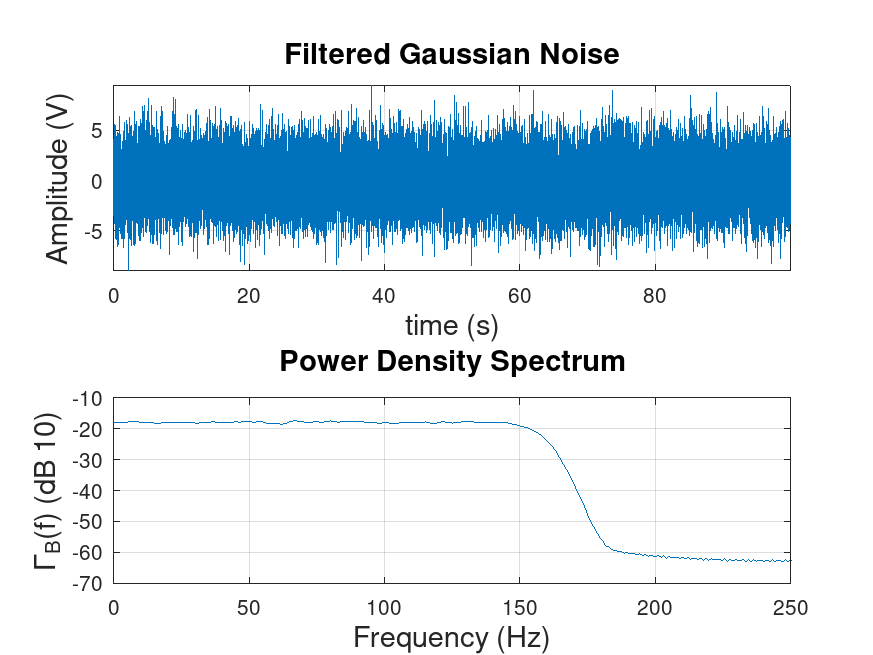
\includegraphics[width=\columnwidth]{CGN.png}
\caption{Réalisation et densité spectrale de puissance moyenne  du bruit: $B=160~Hz$, $P_B= 5~V^2$, $\sigma_B = \sqrt{5}$, $\mu_B=0$.}
\label{fig-B}
\end{figure}
\finrep

\begin{table}[H]
\begin{center}
\begin{tabular}{| L{40mm} | C{40mm}|}\hline
Moyenne $B(t)$ 		
& $-1.854294e-17}$ 	
\\[5mm] \hline
Variance $B(t)$
& $5$
\\[5mm] \hline
\end{tabular}
\end{center}
\label{table-B}
\caption{Mesures de la moyenne et de la variance de $B(t)$.}
\label{tab-B}
\end{table}



A partir  de la Figure \ref{fig-B} et en expliquant la démarche suivie, retrouver (approximativement) la valeur de $\Gamma_0$. Comparer à la valeur théorique de la préparation.

\debutrep{réponse ci-dessous}
Pour retrouver graphiquement la valeur on regarde la valeur moyenne en bande passante, on inverse ensuite l'échelle logarithmique.

On mesure $10\log_{10}(\Gamma_0)\approx -18$
On a alors
\[
\Gamma_0 = 10^{\frac{-18}{10}} \approx 0.0158
\]

On retrouve alors la valeur théorique.
\finrep

\subsection{Etude du filtre passe-bande $\mathcal{F}_1$}
\label{sec:bruit-passe-bande}

On filtre le bruit $B(t)$ par un filtre passe-bande, de bande passante  $\Delta\nu$ centrée sur  la fréquence  $F_0$. 

\subsubsection{}

On choisit $\Delta\nu = \dnu~Hz$ et la valeur de $F_0$ identifiée dans la préparation.  \\
Reproduire dans le cadre ci-dessous, le code permettant de:
\begin{list}{-}{\setlength{\leftmargin}{3mm} \setlength{\labelwidth}{20mm} \setlength{\labelsep}{2mm} \setlength{\itemsep}{1mm} }
\item synthétiser le filtre $\mathcal{F}_1$ correspondant
\item filtrer le bruit $B(t)$ par le filtre $\mathcal{F}_1$ (afficher avec des légendes pertinentes, la sortie du {\tt BPF.m} dans la Figure \ref{fig-Y}) 
\item de mesurer sur la trace en sortie du filtre $\mathcal{F}_1$ les valeurs des paramètres demandés dans la \textbf{Table  \ref{table-YB}} (reporter ces valeur mesurées dans la \textbf{Table \ref{table-YB}}):
\end{list}

\debutrep{code ci-dessous}
\begin{verbatim}
order = 6 % Ordre du filtre butterworth (butter)
dnu = 16  % Hz

Fp = struct('Fs', Fs,
            'F0', nu0,
            'Dnu', dnu,
            'order', order,
            'class', 'bandpass'
            );
[Y, Fp] = BPF(X, Fp);

disp(sprintf("Moyenne de YB(t): %d", mean(Y.data)));
disp(sprintf("Variance de YB(t): %d", std(Y.data)^2));
\end{verbatim}
\finrep

\debutrep{figure ci-dessous}
\begin{figure}[H]
\centering
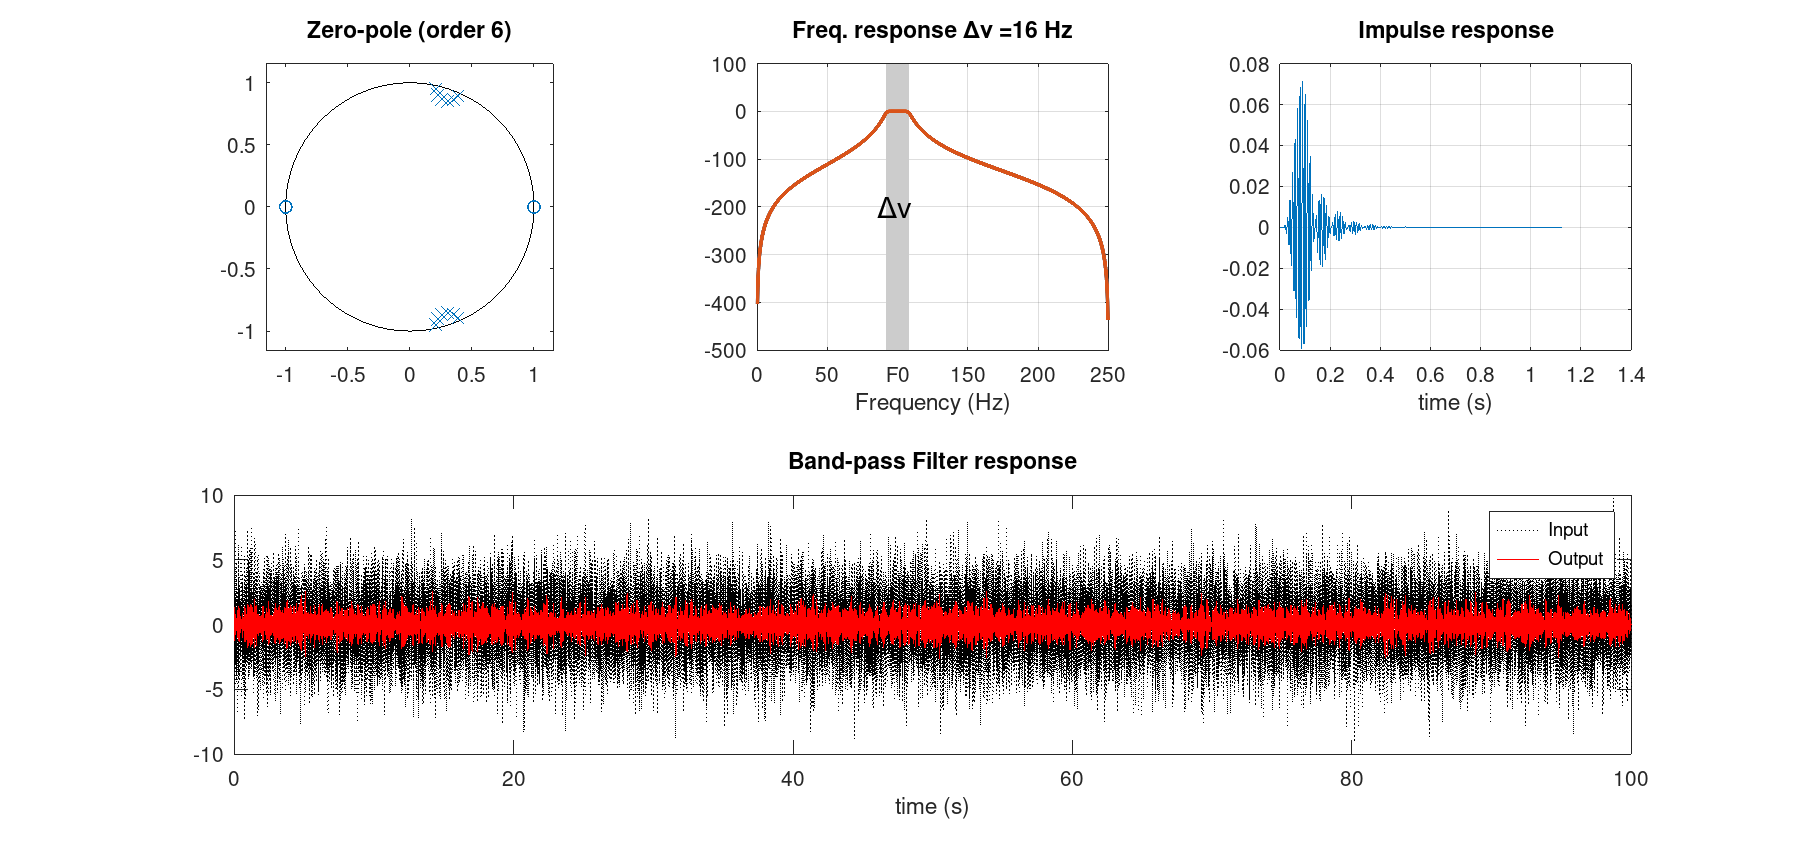
\includegraphics[width=1.1\columnwidth]{BPF.png}
 \caption{Bruit Y(t) filtré passe-bande pour $\Delta\nu = \dnu$ Hz}
 \label{fig-Y}
\end{figure}
\finrep

\begin{table}[H]
\begin{center}
\begin{tabular}{| L{40mm} | C{40mm}|}\hline
Moyenne $Y_{B}(t)$ 	
& $1.423847e-05$
\\[5mm] \hline
Variance $Y_{B}(t)$ 	
& $4.623888e-01$
\\[5mm] \hline
\end{tabular}
\end{center}
\caption{Mesures de la moyenne et de la variance de $Y_{B}(t)$.}
\label{table-YB}
\end{table}

\subsubsection{}

Estimer la valeur de $\Gamma_0$. Comparer les mesures ($\overline{P}_{Y_B}$ et $\Gamma_0$) aux valeurs théoriques obtenues en préparation. Comment peut on expliquer les éventuelles différence?

\debutrep{réponse ci-dessous}
    \begin{gather}
        \nonumber \overline{P}_Y_B = \sigma^2_Y_B \approx 0.465326 \\
        \nonumber \Gamma_0 = \frac{\overline{P}_Y_B}{2*\Delta\nu} \approx 0.0145414
    \end{gather}
\finrep

\subsubsection{}
En pratique, qu'est ce qui limite le choix d'une  bande passante $\Delta \nu$ trop étroite?

\debutrep{réponse ci-dessous}
Une bande passante $\nu$ très étroite dans le domaine spectrale correspond à une bande d'autant plus étendue dans le domaine temporelle.

Une réponse impulsionnelle très longue signifie alors que pour que le filtre fonctionne à plein régime, on doit attendre au moins autant d'échatillons que de points de la réponse impulsionnelle.

Les premiers échantillons sont donc erronés et si la longueur de la réponse impulsionnelle vient à dépasser le nombre de points du signal, le signal en sortie sera alors totalement erroné.
\finrep


\subsection{Elévation au carré et Filtrage RC passe-bas}

\subsubsection{}

Comme précédemment, on choisit $\Delta\nu = \dnu Hz$. En faisant varier le produit $\Delta \nu \times RC$ dans une boucle (du type {\tt for \ldots end}), donner dans le cadre ci-dessous, le code qui:

\begin{list}{-}{\setlength{\leftmargin}{3mm} \setlength{\labelwidth}{20mm} \setlength{\labelsep}{2mm} \setlength{\itemsep}{1mm} }
\item génère le signal $Z_B(t)= Y_B^2(t)$ 
\item calcule la valeur de la constante $RC$ correspondant au produit $\Delta\nu \times RC$ choisi
\item filtre le signal $Z_B(t)$ par le filtre $\mathcal{H}_{I}$ de constante de temps $RC$  
\item mesure sur la sortie $W_B(t)$ les paramètres demandés dans la  \textbf{Table \ref{table-WB}} (y reporter les valeurs mesurées)
\end{list}

\debutrep{code ci-dessous}
\begin{verbatim}
%%%%%%%%%%%%%%%%%% 1.3 Filtrage passe bande %%%%%%%%%%%%%%%%%%%

Z = struct('data', Y.data.^2, 'time', Y.time, 'Fs', Y.Fs);

product = [2,20,100];
for i=1:3
  
  RC = product(i)/dnu;
  fprintf("-----> Produit RC*dnu = %d\n", product(i));
  
  figure()
  RCFp = struct('Fs', Fs, 'RC', RC);
  [W, RCFp] = RCF(Z, RCFp);

  fprintf("RC: %f", mean(RC));
  fprintf("Moyenne de YB(t): %f\n", mean(Wb.data));
  fprintf("Variance de YB(t): %f\n", std(Wb.data)^2);
  fprintf("Kurtosis de YB(t): %f\n", kurtosis(Wb.data));
  
  WC = W.data( W.time > round(RC*5));
  
  fprintf("Moyenne corrigée de W(t): %f\n", mean(WC));
  fprintf("Variance corrigée de W(t): %f\n", std(WC)^2);
  fprintf("Kurtosis corrigée de W(t): %f\n", kurtosis(WC));
  
end
\end{verbatim}
\finrep

Remplir le tableau de mesures de la Table \ref{table-WB} (ignorez dans un premier temps les mesures demandées {\em après correction}).

\begin{table}[h]
\begin{tabular}{| L{40mm} | C{35mm} | C{35mm} | C{35mm} |}\hline
$\Delta\nu \times RC$ 
& 2 
& 20 
& 100 \\[5mm]  \hline\hline
$RC$ 
& $0.125$
& $1.25$ 
& $6.25$
\\[5mm]  \hline \hline
moyenne $W_B(t)$ 	
& $0.461849$
& $0.469187$	
& $0.414726$	 
\\[5mm] \hline
variance $W_B(t)$ 	
& $0.045280$
& $0.005972$	
& $0.011692$	
\\[5mm]  \hline
Kurtosis $W_B(t)$ 	
& $5.395773$	
& $2.961607$	
& $2.630713$	 
\\[5mm]  \hline \hline
moyenne $W_B(t)$ \newline (après correction) 	
& $0.462742$	
& $0.478302$	
& $0.467627$	
\\[5mm] \hline
variance $W_B(t)$\newline (après correction) 	
& $0.044947$	
& $0.003816$	
& $0.000265$	
\\[5mm]  \hline
Kurtosis $W_B(t)$\newline (après correction)	
& 4.740478	
& 3.347973	
& 3.653368	
\\[5mm]  \hline
\end{tabular}
\caption{Sortie Filtre $RC$ - Cas du bruit seul.}
\label{table-WB}
\end{table}

\subsubsection{}
Le processus $Z_B(t)$ (\textbf{signal en sortie du quadrateur}) est-il gaussien? Pourquoi?

\debutrep{réponse ci-dessous}
On observe que pour un produit $RC\times\Delta\nu$ est grand, plus le kurtosis du signal se rapproche de 3, c'est à dire plus il se rapproche d'une répartition gaussienne.

Celà s'explique par le caractère intégrateur du filtre RC. On peut voir cette intégration comme une somme continue de tirages de la variable aléatoire $Z_B(t)$. Cette somme est d'autant plus grande que RC est grand.
Le signal étant stationnire, toutes ces variables obéissent à la même loi $Z_B(t)$.

Le théorème central limite nous dit donc que plus on somme de variables aléatoire suivant la même loi, plus la somme finale tend vers une répartition gaussienne.
\finrep

\subsubsection{}
Pour les 2 valeurs extrêmes de $\Delta\nu \times RC$ proposées dans la Table \ref{table-WB}, afficher dans la Figure ci-dessous, les sorties de {\tt RCF.m}.

\debutrep{figure ci-dessous}
\begin{figure}[H]
\begin{tabular}{cc}
(a) 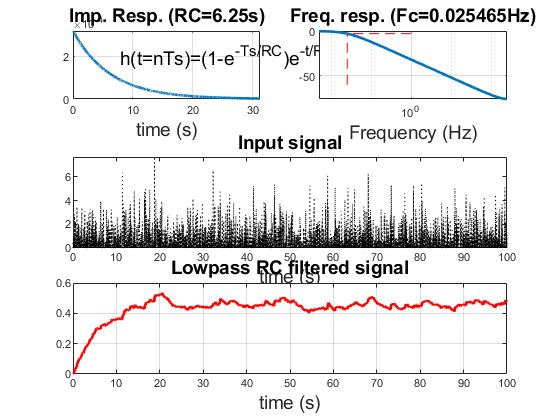
\includegraphics[width=0.85\columnwidth]{RCnu-MAX.png} \\
(b) 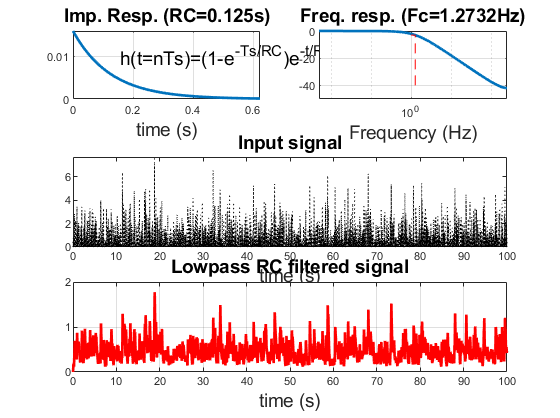
\includegraphics[width=0.85\columnwidth]{RCnu-MIN.png} 
\\
\end{tabular}
 \caption{Sortie $W_B(t)$ du filtre passe-bas pour $\Delta\nu = 16$ Hz -- 
  (a) $RC$ = 12.5. ($\Delta\nu\times RC=200 $) (b) $RC = 0.125 $ ($\Delta\nu\times RC = 2 $) }
 \label{fig-Wb}
\end{figure}
\finrep


\subsubsection{}

Comparer pour chaque valeur de la constante $RC$, la valeur moyenne mesurée à la valeur théorique déterminée dans la préparation. Qu'est ce qui peut expliquer ces différences? Comment corriger cet effet?  \\

\debutrep{réponse ci-dessous}
On observe pour une valeur de RC importante, on observe une "pente" à l'origine avant que le signale se stabilise avec une valeur moyenne plus éloignée de la puissance moyenne que dans les autres cas.

Dans le cas d'une valeur RC plus faible, on observe une forte variabilité du signal de sortie. On obtiens en revanche une "pente" à l'origine bien plus faible que les autres cas et donc une valeur moyenne plus proche de la valeur de la puissance moyenne.
\finrep

\subsubsection{}
Donner dans l'encadré ci-dessous les 2 lignes de code qui implémentent cette solution.

\debutrep{code ci-dessous}
\begin{verbatim}
WC = W.data( W.time > round(RC*5));
\end{verbatim}
\finrep

Appliquer cette correction et porter les nouvelles mesures dans la Table \ref{table-WB} (partie {\em avec correction}).


\subsubsection{}
Lorsque le Kurtosis est proche de $3$, que peut on dire de la statistique du processus $W_B(t)$? \\
\textbf{Quel théorème important ce résultat illustre-t-il?}\\
 Pour quelles(s) valeur(s) de $RC$ a-t-on une {\em intégration forte}?  Comparer les variances de $W_B(t)$ mesurées pour les deux valeurs extrêmes de $RC$. 

\debutrep{réponse ci-dessous}
Lorsque le Kurtosis est proche de 3, le processus aléatoire s'assimilie à un processus gaussien.

Une intégration est une somme continue d'une multitude de points, étant chacun une variable aléatoire (et suivant la même loi si stationnaire).
Le Théorème Central Limite permet donc de dire que cette intégrale s'approchera d'une répartition gaussienne.\\
\\
On a une intégration forte si $RC \gg \frac{1}{\Delta\nu}$ c'est à dire $RC \gg 1/16 \approx 0.0625$. \\
On a donc une forte intégration pour $RC = 1.25$ et  $RC = 6.25$.\\
\\

Un filtre intégrateur est un filtre moyenneur, on observe alors une forte diminution de la variance pour un $RC$ grand.\\
$W_b(t) (RC = 0.125) \gg W_b(t) (RC=6.25)$

\finrep

\textbf{Dans la suite du TP, il faudra systématiquement appliquer cette correction aux mesures effectuées en sortie du filtre RC.}

\clearpage
\section{Mélange Signal + Bruit}
\label{sec:melange}

On étudie à présent le signal $W(t)$ en sortie du filtre RC passe-bas, lorsque le mélange $X(t) = S(t) + B(t)$ est reçu en entrée du détecteur.

\subsection{Sortie du filtre passe-bande $\mathcal{F}_1$}

\subsubsection{}

En utilisant  les paramètres déterminés en préparation, générer une réalisation du signal $S(t)$ sur la même durée $T=100~s$ et la même fréquence d'échantillonnage $F_s = 500~Hz$. \\[1mm]
Reporter le code correspondant ci-dessous.

\debutrep{code ci-dessous}
\begin{verbatim}
t = 0:1/Fs:T-1/Fs;   % Vecteur temps de 0 à T secondes

  % Message
A0 = 1;
phi = rand() * 2*pi;  % Phase aléatoire
M = 0;

S = M*A0*cos(2*pi*nu0*t + phi);
\end{verbatim}
\finrep

 
\subsubsection{}

Vérifier que le filtre passe-bande, s'il est accordé sur la fréquence $\nu_0$ n'altère pas le  signal $S(t)$, en mesurant en sortie de $\mathcal{F}_1$ (dans le cas où $S(t)$ se présente seul en entrée) les paramètres demandés à la \textbf{Table \ref{table-YSB}}. En reprenant les mesures  effectuées au paragraphe \ref{sec:bruit-passe-bande}, déterminer le rapport signal sur bruit $\eta_{E_1}$ en sortie du sortie du filtre $\mathcal{F}_1$ ainsi que le gain $\eta_{E_1}/\eta_E$ introduit par $\mathcal{F}_1$.


\begin{table}[H]
\begin{center}
\begin{tabular}{| L{40mm} | C{40mm}|}\hline
Fréquence $Y_{S}(t)$ 		& 100Hz 	\\[5mm] \hline
Amplitude $Y_{S}(t)$ 		& 0.996	\\[5mm] \hline
Puissance  $Y_{S}(t)$ 		& 4.998797e-01	\\[5mm] \hline
Puissance  $Y_{B}(t)$  \newline
(recopie Table \ref{table-YB}) &  0.465	\\[5mm] \hline
SNR $\eta_{E_1}$ 
& $\frac{\overline{P}_Y_S} {\overline{P}_Y_B}\approx 1.075268817$	
\\[5mm] \hline
Gain $\eta_{E_1}/\eta_E$ 	
& 	$\frac{1.0753}{0.1} \approx 10.8$
\\[5mm] \hline
\end{tabular}
\end{center}
\caption{Mesures des SNR et gains en sortie de $\mathcal{F}_1$.}
\label{table-YSB}
\end{table}

\subsubsection{}

Comparer aux valeurs théoriques.

\debutrep{réponse ci-dessous}
Les résultats trouvés sont en adéquation avec la théorie.
\finrep

\subsection{Sortie du filtre RC passe-bas}

\subsubsection{}

Dans les mêmes conditions expérimentales  ($\overline{P_B} = 5~V^2$,  $\Delta\nu = \dnu Hz$, $\eta_E=-10~dB=0.1$), effectuer les différentes mesures demandées dans \textbf{la table \ref{table-WSB}}. 

\begin{table}[H]
\begin{tabular}{|L{6mm}| L{40mm} | C{35mm} | C{35mm} | C{35mm} |}\hline
	& $\Delta\nu \times RC$ 		& 2 	& 20 	& 100 \\[5mm]  \hline
	& $RC$ 					
 & 	0.125
 &	1.25
 &	6.25
 \\[5mm]  \hline \hline
T	& $S_S$ 					
&	0.5
&	0.5
&	0.5
\\[5mm]  \cline{2-5} % \hline
H	& $B_S=\mathbb{S}td\{W_{S+B}\}$ 
&	0.433
&	0.137
&	0.061
\\[5mm]  \cline{2-5} %  \hline
É	& SNR $\eta_S$				
&	0.41
&	3.65
&	8.17
\\[5mm]  \cline{2-5} %  \hline 
O	& Gain $g_1$				
&	1.16
&   3.65
&	8.16
\\[5mm] \cline{2-5} % \hline
. 	& Gain $g$ 				
&	11.54
&	39.5
&	81.61
\\[5mm]  \hline\hline
M 	& moyenne $W_B$ \newline 
(recopie de Table \ref{table-WB}) 		
& $0.462742$	
& $0.478302$	
& $0.467627$	
\\[5mm]  \cline{2-5} %\hline
E 	& moyenne $W_{S+B}$  		
&	0.963213
&	0.958718
& 	0.960965
\\[5mm]  \cline{2-5} %\hline
S 	& $S_S$ 					
&	0.500471
&	0.480416
&	0.493338
\\[5mm]  \cline{2-5} %\hline
U 	& $B_S=\mathbb{S}td\{W_{S+B}\}$ 
&	0.383289
&	0.125912
&	0.044490
\\[5mm]  \cline{2-5} % \hline
R 	& SNR $\eta_S$ 				
&	1.305727532
&	3.815490184
&	11.088739042
\\[5mm]  \cline{2-5} % \hline
E
&   Gain $g_1 = \frac{\eta _S}{\eta _E_1}$ 				
&   1.2143
&	3.5484
&	10.3125
\\[5mm]  \cline{2-5} %\hline
S 	& Gain $g = \frac{\eta _S}{\eta _E}$ 				
&	13.05727532
&	38.15490184
&	110.88739042
\\[5mm]  \hline\hline
\end{tabular}
\caption{Sortie Filtre $RC$ - Cas du mélange signal $+$ bruit.}
\label{table-WSB}
\end{table}


\subsubsection{}

Représentez dans la Figure \ref{fig-Wsb}, la sortie de {\tt RCF.m} correspondant au cas  $\Delta\nu \times RC = 20$.

\debutrep{figure ci-dessous}
\begin{figure}[H]
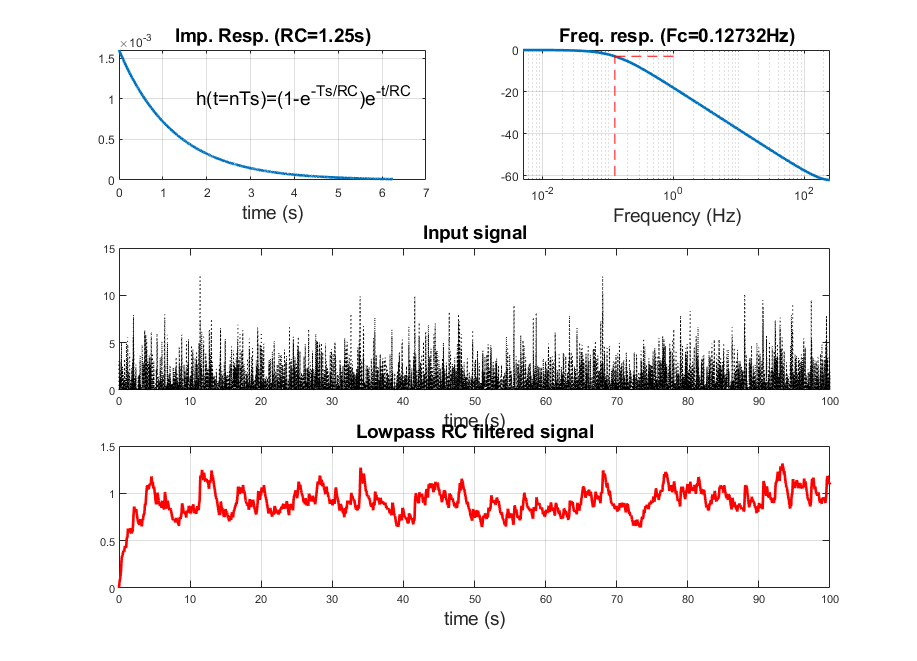
\includegraphics[width=\columnwidth]{RCnu20-S+B.png}
\caption{Signal $W_{S+B}(t)$ dans le cas du mélange signal + bruit ($\Delta \nu = 16$ Hz, $\Delta\nu \times RC = 20$)}
\label{fig-Wsb}
\end{figure}
\finrep

\clearpage

\section{Transmission d'un message binaire}

\subsection{Modulation binaire périodique}

On souhaite à présent transmettre et détecter une séquence périodique binaire.\\

\subsubsection{}

Avec les paramètres suivant:\\[-3mm]
\begin{list}{-}{\setlength{\leftmargin}{3mm} \setlength{\labelwidth}{20mm} \setlength{\labelsep}{2mm} \setlength{\itemsep}{1mm} }
\item[--] Puissance du bruit $B(t)$, $\overline{P}_{B}  = 5~V^2$
\item[--] Rapport signal sur bruit en entrée de la chaine, $\eta_E = -10~dB$
\item[--] Fréquence du signal modulant $M(t)$, $F_M = 0.05~Hz$
\item[--] Durée des signaux, $T = 100~s$\\[-2mm]
\end{list}

synthétiser les  signaux $S(t)$,  $B(t)$ et $X(t)$ correspondant. \\

En vous basant sur les résultats expérimentaux obtenus dans la partie \ref{sec:melange}, choisissez un jeu de paramètres pertinent pour calibrer les filtres 
$\mathcal{F}_1$ et $\mathcal{H}_I$. Reporter dans le cadre ci-dessous le code  de détection du signal binaire reçu. 

\debutrep{code ci-dessous}
\begin{verbatim}

signal = WC.data > mean(WC.data);

\end{verbatim}
\finrep

\subsubsection{}

Visualiser dans la Figure \ref{fig-binaire}  (en organisant avec la commande {\tt subplot(4,1,$\cdot$)} et en ajoutant une légende pertinente), les signaux:\\[-3mm]
\begin{list}{-}{\setlength{\leftmargin}{3mm} \setlength{\labelwidth}{20mm} \setlength{\labelsep}{2mm} \setlength{\itemsep}{1mm} }
\item[--] $S(t)$
\item[--] $X(t)$
\item[--] $W(t)$
\item[--] Le signal binaire détecté obtenu par seuillage du signal $W(t)$ (commenter le choix du seuil $\Sigma$ choisi)
\end{list} 

\debutrep{figure ci-dessous}
\begin{figure} [H]
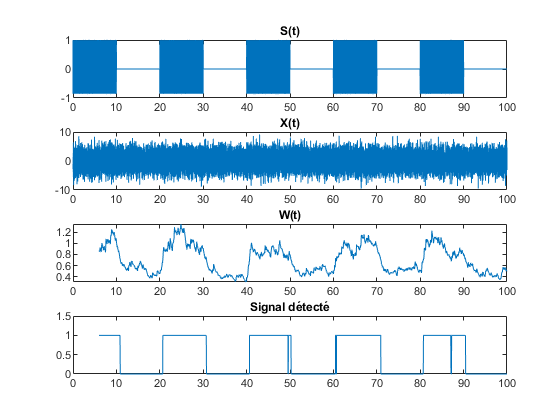
\includegraphics[width=\columnwidth]{4plots.png}
\caption{(a) Signal binaire $S(t)$. (b) Mélange Signal (binaire) + bruit avant et apres filtrage passe-bande. (c) Sortie $W(t)$ de la chaine de détection quadratique. (d) Signal binaire détecté après seuillage de la sortie quadratique.}
\label{fig-binaire}
\end{figure}

Le seuil est défini à la valeur moyenne du signal $W(t)$ pour se placer au plus proche de la moyenne du signal émis et ainsi avoir le minimum d'impact du bruit sur le signal.


\finrep


\subsubsection{}

Indiquez les valeurs des paramètres de détection utilisés.

\debutrep{réponse ci-dessous}
\begin{center}
    \begin{cases}
    $\Delta \nu = 16$ Hz \\
    $RC\Delta\nu = 20$
    \end{cases}
\end{center}
\finrep

\subsubsection{}

Essentiellement quel élément de la chaine de détection va-t-il limiter le débit de transmission?

\debutrep{réponse ci-dessous}
La vitesse de charge / décharge du condensateur va limiter la vitesse de transmission. Il faudrait alors changer la valeur de le constante de temps RC pour s'adapter à ce changement de débit.
\finrep

\subsubsection{}
Sans chercher à les estimer ici, quel(s) critère(s) permettrai(en)t de mesurer la qualité de la détection?

\debutrep{réponse ci-dessous}
Il faudrait vérifier la valeur maximale coefficient de corrélation entre le signal émis et le signal reçu, permettant de juger l'intégrité du signal transmi.
On pourrait également s'intéresser aux proriétés statisques des signaux d'entrée et de sortie (éspérance, variance, kurtosis, puissance moyenne) pour vérifier les impacts de la transmission.
\finrep


\subsection{Décodage d'un message inconnu}


Charger le signal reçu {\tt 'SignalRecu\_j'}, où $j$ est le numéro de votre binôme.\\[2mm]
{\tt >\!> load SignalRecu\_1}\\[2mm]
Le signal $X(t)$ correspond à un message codé (code ascii 7 bits) transmis par modulation d'amplitude et  dégradé par un bruit additif lié au canal de transmission. 
Exécuter  la  commande: \\[2mm]
{\tt >\!> [TxMsg,Xp] = RxMessage\_DQ(X,Xp) ; }  \\[2mm]
pour lancer une détection quadratique {\em automatique} sur le signal reçu $X$ (la structure $Xp$ contient tous les paramètres de la transmission).
Ajuster en ligne, les différents paramètres de la détection jusqu'à ce que le message décodé vous semble satisfaisant. Recopier ci-dessous, le message décodé. 

\debutrep{réponse ci-dessous}
On travaille avec le signal numéro 2.\\
\\
Les paramètres utilisés pour la détection sont:
\begin{cases}
    \delta\nu = 16\\
    RC\Delta\nu = 20 \\
    \Sigma = 0.5
\end{cases}\\
\\
Le message reçu sur le signal "SignalRecu\_2.mat" est "Nous disons: Tante Amelie fait du velo en short".
\finrep

\end{document}
































